\documentclass[12pt, a4paper, titlepage]{article}

\usepackage[utf8]{inputenc}     % Permite el uso de caracteres como ñ y acentos
\usepackage[spanish]{babel}     % Configura el documento en español
\usepackage{graphicx}           % Para manipular gráficos e imágenes en el documento
\usepackage{float}              % Permite forzar una ubicación exacta de imágenes con [H]
\usepackage{listings}           % Permite formato de fragmentos de código de programación
\usepackage[autostyle=false, style=english]{csquotes} % Permite escribir "" con \enquote{}
\usepackage[explicit]{titlesec} % Permite personalizar el estilo de los títulos y secciones
\usepackage{xcolor}             % Para definir y usar colores personalizados en texto
\usepackage{geometry}           % Para configuración de los márgenes y el tamaño de la página
\usepackage{lipsum}             % Para generar texto de relleno ("Lorem ipsum")
\usepackage{tocloft}            % Para personalizar el formato del índice
\usepackage{subfiles}           % Para incluir de otros archivos .tex en el main mediante \include{}
\usepackage[colorlinks=true, allcolors=blue, linktoc=all]{hyperref} % Crea enlaces dentro del documento 
\usepackage{bookmark}           % Mejora la administración de los marcadores (bookmarks) en documentos PDF generados
\usepackage{xr}                 % Permite referenciar elementos de otros documentos .tex
\usepackage{natbib}             % Para gestionar bibliografías y hacer citaciones



% Configuración de márgenes
\geometry{
    left=2.5cm,  % Margen izquierdo
    right=2.5cm, % Margen derecho
    top=3cm,     % Margen superior
    bottom=3cm   % Margen inferior
}


% Definimos una nueva forma de referirnos a las \section, \subsection y \subsubsection.
% Ahora en los subarchivos tex al llamarlas de esta forma aseguramos que en la
% Table of Contents (ToC) aparezcan los números de las secciones que seleccionemos
%     \subsection*{} hace que salga el titulo en formato subsection pero no aparece en el ToC
%     \numberedsubsection hará que si salga en la ToC


% ESTA VERSION NO TIENE NÚMEROS EN LOS TÍTULOS     Section, Subsection... 
\newcommand{\numberedsection}[1]{%
  \stepcounter{section}%
  \section*{#1}%
  \addcontentsline{toc}{section}{\protect\numberline{\thesection}#1}%
}
\newcommand{\numberedsubsection}[1]{%
  \stepcounter{subsection}%
  \subsection*{#1}%
  \addcontentsline{toc}{subsection}{\protect\numberline{\thesubsection}#1}%
}
\newcommand{\numberedsubsubsection}[1]{%
  \stepcounter{subsubsection}%
  \subsubsection*{#1}%
  \addcontentsline{toc}{subsubsection}{\protect\numberline{\thesubsubsection}#1}%
}

% ESTA VERSIÓN LE PONE NÚMEROS A LOS TÍTULOS:   1. Section, 1.1 Subsection... 
% \newcommand{\numberedsection}[1]{
%   \stepcounter{section}
%   \section*{\thesection\hspace{0.5em}#1}
%   \addcontentsline{toc}{section}{\protect\numberline{\thesection}#1}
% }

% \newcommand{\numberedsubsection}[1]{
%   \stepcounter{subsection}
%   \subsection*{\thesubsection\hspace{0.5em}#1}
%   \addcontentsline{toc}{subsection}{\protect\numberline{\thesubsection}#1}
% }

% \newcommand{\numberedsubsubsection}[1]{
%   \stepcounter{subsubsection}
%   \subsubsection*{\thesubsubsection\hspace{0.5em}#1}
%   \addcontentsline{toc}{subsubsection}{\protect\numberline{\thesubsubsection}#1}
% }

% Definimos comando para realizar un tab
\newcommand\tab[1][1cm]{\hspace*{#1}} 

% Definimos forma de llamar al listado con letras minúsculas pero sustituye el listado por 
% números de enumerate. Comentar para tener enumerate por default.
% \renewcommand{\theenumi}{\alph{enumi}}
% \begin{enumerate}
%   \item
% \end{enumerate}


% Configuración para sintaxis usando código VHDL
\lstdefinestyle{Código_VHDL}{
    language=VHDL,                % Especifica VHDL como el lenguaje
    basicstyle=\ttfamily\small,   % Estilo básico: letra monoespaciada pequeña
    keywordstyle=\color{red!90!black}, % Color para palabras clave
    commentstyle=\color{green!50!black}, % Color para comentarios
    tabsize=2,                    % Tamaño del tabulador
    showspaces=false,             % No mostrar espacios
    showstringspaces=false,       % No mostrar espacios en cadenas de texto
    breaklines=true,              % Ajustar líneas largas
}

\begin{document}

% PORTADA
\begin{titlepage}
  \centering
  {\bfseries\LARGE Universidad de Málaga\par}
  \vspace{1cm}
  {\scshape\Large ETSI Informática\par}
  \vspace{2cm}
  {\scshape\Huge Diseño orientado a objetos\par}
  \vspace{0.1cm}
  {\scshape\Huge de un refugio de animales}
  \vspace{2cm}
  \begin{figure}[H]
      \centering
       
\includegraphics[width=0.30\linewidth]{assets/umaLogo.png}
  \end{figure}
  \vfill
  {\scshape\Large Modelado y Diseño del Software (2024$-$25)\par}
  \vspace{0.5cm}
  {\Large Daniil Gumeniuk\par}
  {\Large Angel Bayon Pazos \par}
  {\Large Diego Sicre Cortizo\par}
  {\Large Pablo Ortega Serapio\par}
  {\Large Angel Nicolás Escaño López\par}
  {\Large Francisco Javier Jordá Garay\par}
  {\Large Janine Bernadeth Olegario Laguit\par}
  \vspace{1cm}
  {\Large Grupo 1.1}
  \vfill
  {\Large Diciembre 2024}
  
  \end{titlepage}
% FIN PORTADA  

% ÍNDICE
\tableofcontents % Crea el Índice
\thispagestyle{empty} % Quita el número de la primera página
\addtocontents{toc}{\protect\thispagestyle{empty}} % Asegura que cada página del índice sea sin número de página

\newpage

\listoffigures % Crea un Índice de Figuras (registra imágenes)
\thispagestyle{empty}
\addtocontents{lof}{\protect\thispagestyle{empty}}

\newpage
% FIN ÍNDICE


% RESUMEN
\thispagestyle{empty}
\begin{abstract}
  Esta práctica aborda el diseño e implementación de un sistema orientado a objetos para 
  gestionar un refugio de animales utilizando Java y conceptos de diseño orientado a objetos 
  vistos en el Tema 5.\par
  \vspace{0.5cm}
  El objetivo principal es analizar las posibles estrategias de diseño que permitan implementar 
  este modelo, abordando desafíos como la necesidad de que un mismo socio pueda desempeñar múltiples 
  roles simultáneamente.
  
  A lo largo del documento se discute por qué las clases descritas inicialmente no pueden ser implementadas 
  directamente en Java y se propone una posible solución mediante técnicas como composición, interfaces, y herencia 
  múltiple simulada para garantizar la consistencia del sistema.\par
  \vspace{0.5cm}
  Finalmente, la solución propuesta acompañada de un diagrama de diseño que ilustra la arquitectura del sistema, 
  muestra la reutilización de métodos, la integridad de los datos y la flexibilidad necesaria para adaptarse a 
  los requerimientos del modelo conceptual.\par
\end{abstract}

\newpage
% FIN RESUMEN


% CUERPO DEL DOCUMENTO
\setcounter{page}{4} % Inicia a contar las páginas a partir de {}

\section{Ejercicio 3}
\subsection*{Instrucción}
Cuando los clientes de la empresa de alquiler de coches alquilan un coche, el sistema que estamos construyendo
tiene que proporcionarles el precio del alquiler. Este precio lo calcula la operación \texttt{getPrice() : Integer} de la siguiente
forma: El precio base será el precio del modelo del vehículo por día.
\begin{center}
    \texttt{ (pricePerDay) * [endDate - startDate]}
\end{center}
Además, la empresa de alquiler de coches puede añadir al cálculo de precios la posibilidad de hacer promociones
que implican descuentos de estos precios. Inicialmente, la empresa ofrecerá dos tipos de promociones: por cantidad
y por porcentaje.
\begin{itemize}
    \item \textbf{Promoción por cantidad:} permitirá decrementar el precio del alquiler en la cantidad indicada en
    la promoción.
    \item \textbf{Promoción por porcentaje:} decrementará el precio del alquiler en el porcentaje indicado en la
    promoción. Las promociones se asignan a los alquileres en el momento de su creación.
\end{itemize}
Evidentemente, es posible
que a algunos alquileres no se les aplique ninguna promoción. Las promociones que se asignan a los alquileres son
determinadas por una política de la empresa que no impacta al diseño de nuestra operación (impactará a la
operación que crea los alquileres).\par
\vspace{0.15cm}
Eso sí, la empresa quiere que mientras no se haga el pago del alquiler, si aparecen
nuevas promociones, se apliquen a los alquileres siempre y cuando sean más favorables (no nos tenemos que
preocupar tampoco de estos cambios, son gestionados por otras operaciones).


\subsection{Patrón de Diseño utilizado}
Para poder realizar este apartado optamos varias casuisticas de diferentes patrones de diseño validos. Por un lado optamos por el patron visitante,
dicho patron complicaria demasiado la imlementación de la operacion debido al gran numero de instancias presentes de dicho patron para un unico metodo,esto hace que 
el uso de este patron sea algo ineficiente. Tras ese planteamiento llegamos a la conclusion de utilizar el patron \textbf{Strategy} para poder implementar la operacion correctamente.
Este patron se basa en la utilizacion de una interfaz que actua como padre de todos los objetos que implementen una operacion similar, en este caso tenemos dos tipos de promociones,
\textbf{Promoción por porcentaje} y \textbf{Promoción por cantidad} ambas mantienen una logica similar por lo que el uso del patron \textbf{Strategy} es el adecuado.

\subsection{Efectos sobre el Diagrama de Diseño}

\begin{figure}[H]
    \centering
     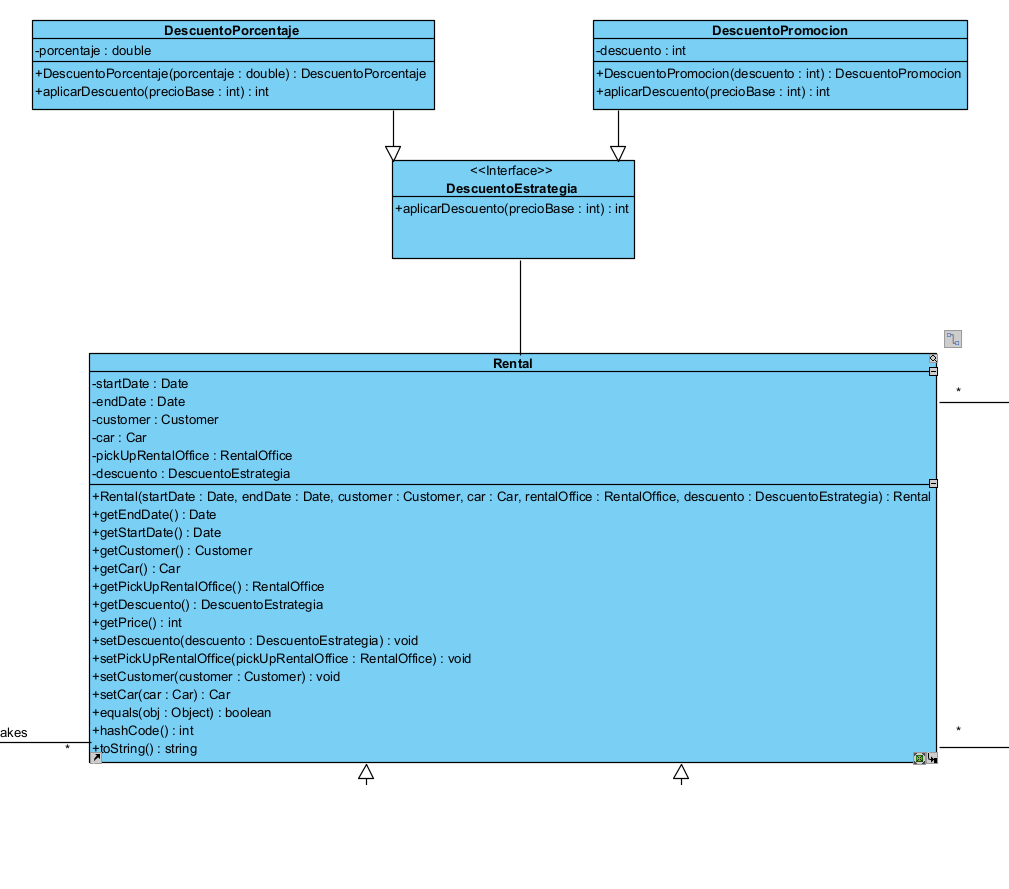
\includegraphics[width=1\linewidth]{assets/diagramas/UML_Apartado3.png}
     \caption{Diagrama de Diseño del apartado 3}
\end{figure}

Como podemos observar, el patron \textbf{Strategy} mantiene una interfaz padre de la cual heredan todas las instancias de objetos que vayan a realizar dicha operacion.
Como bien hemos dicho antes nos basamos en un sistema con dos operaciones diferentes para obtener el precio final, por lo cual necesitaremos crear dos clases una para cada tipo de 
promocion. Estas heredaran de la clase \textbf{Strategy} para asi obligar al sistema a implementar dichas operaciones en cada una de las clases. Un requisito del sistema es que dichas
promociones se apliquen al instanciar un objeto \textbf{Rental}, es por eso que dichos tipos de promociones vendran instanciados en el constructor de dicha clase pudiendo ser nulo en caso 
de que no se le aplique ningun tipo de promocion.\par

\subsection{Implementación de \textit{getPrice() : Integer}}
\begin{lstlisting}[style = javaNormal, language=Java] 

    introducir codigo aqui

\end{lstlisting}\par
En la primera seccion podemos encontrar las nuevas instancias que debemos generar para poder usar el patron \textbf{Strategy} dichas clases implementan el metodo de la interfaz
de manera similar pero cambiando ligeramente la forma en la que calculan los precios a dependiendo de sus propios parametros privados (porcentaje o cantidad).\par
\vspace{0.15cm}
Para implementar el metodo getPrice hemos decidido generar a partir de los parametro \textbf{startDate} y \textbf{endDate} el precio base que tendria el alquiler antes de aplicar 
cualquier tipo de promocion. Como bien hemos explicado antes en caso de que no exista promocion alguna se instanciara como nulo el atributo en el constructor. Es por eso que 
antes de calcular el nuevo precio comprobamos si el \textbf{Rental} contiene un tipo de promocion disponible, en caso contrario devolveremos el precio base inicial.
\newpage



% BIBLIOGRAFÍA
% \newpage

% \addcontentsline{toc}{section}{Referencias}  % Agrega "Referencias" al índice
% \bibliographystyle{apalike}                  % ó elsarticle-num.bst
% \bibliography{citas.bib}                     % Nombre del archivo donde tenemos todas las referencias bibliográficas


\end{document}